\subsection{Dissipative Hamiltonian non equilibrium transformation}
\label{subsec:NISestimators}
%\todo{emphasize on how the choice we take here optimizes the likelihood}
We now return to the challenging target density $\pi(\cdot)= \likelihood(\cdot) \rho(\cdot)/\const$,
where the normalizing constant $\const$ is intractable.  
By applying \Cref{algo:IFIS} to
the test function $\likelihood$, an unbiased estimator of $\const$ is given by
\begin{equation}
  \label{eq:def_estimator_normal_const}
  \estConstC{X^{1:N}}=\frac{1}{N}\sum_{i=1}^{N}
  \sum_{k=0}^K\likelihood(\transfo^{k}(X^i))w_k(X^i) \eqsp.
\end{equation}
\begin{comment}
We  show in Section \ref{subsec:VAE} how this estimator can be used to provide a novel class of Variational AutoEncoder (VAE) using a new evidence lower bound based on the IFIS estimator. 

Let $g$ be a $\pi$-integrable function. To estimate $\int g(x) \pi(x) \rmd x$,  both $\int \likelihood(x) \rho(x) \rmd x$ and  $\int g(x) \likelihood(x) \rho(x) \rmd x$  can be approximated by using \Cref{algo:IFIS} applied to the test functions $\likelihood$ and $ g\likelihood$; \ie~we consider the biased normalized importance sampling estimator $\int g(x) \hatpi{X^{1:N}}(\rmd x)$ where
\begin{align}
  \label{eq:def_estimator_naive_monte_carlo}
  &\hatpi{X^{1:N}}(\rmd x)= \sum_{i=1}^{N}
  \sum_{k\in \zset} p_k^i \updelta_{\transfo^k(X^i)}(\rmd x),\\
  &\text{where}~p_k^i\propto \likelihood(\transfo^{k}(X^i)) w_k(X^i)
  %,~\sum_{i=1}^{N} \sum_{k\in \zset} p_k^i=1 \eqsp.
\end{align}
\end{comment}
The efficiency of such an estimator relies heavily on the choice of $\transfo$. Intuitively, a sensible choice of
$\transfo$ requires that  (i) $\transfo$ is able to drive samples to regions which contributes strongly to the computation of $Z$ (aka regions where the likelihood $\likelihood$ is high) and (ii) that the Jacobian of $\transfo$ is cheap to compute. 
\begin{figure}[ht]
    \centering
    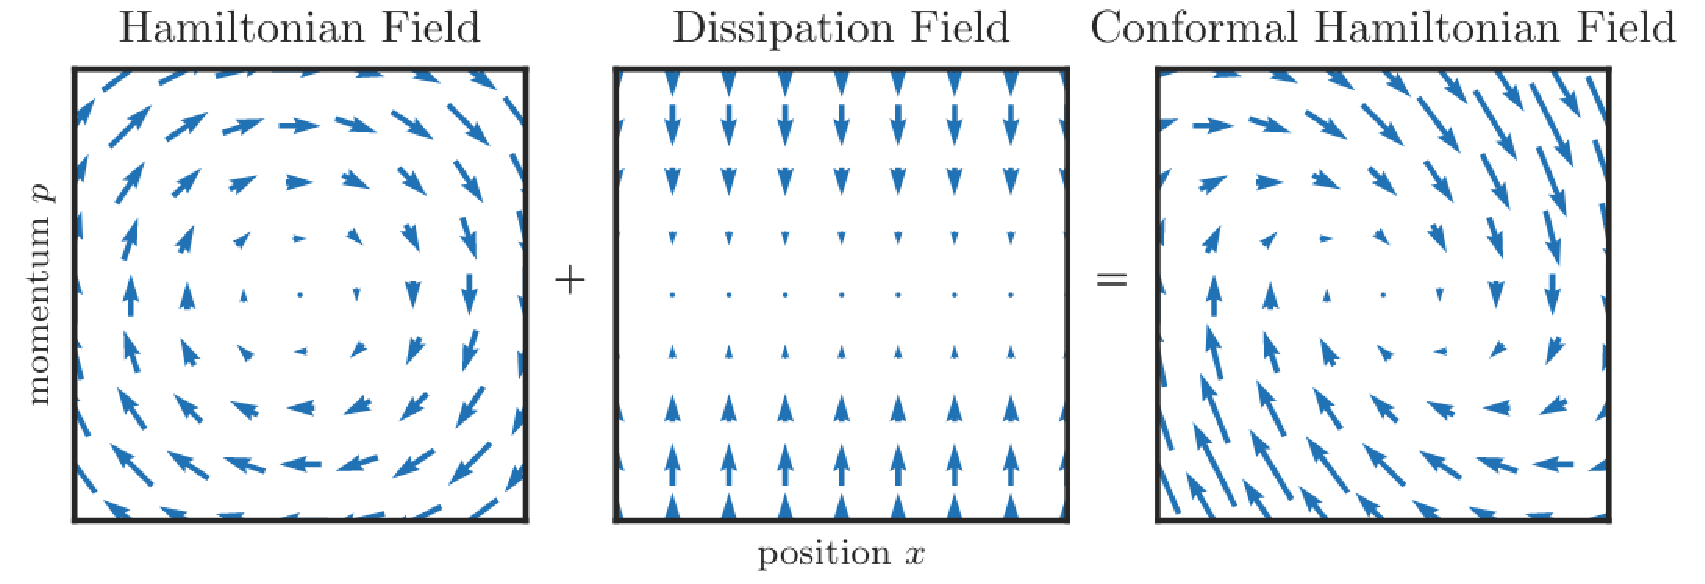
\includegraphics[width=\linewidth]{pics/conformal_hamiltonian.pdf}
    \caption{Representation of the effect of a conformal Hamiltonian on the phase space in 1 dimension, from \cite{maddison2018hamiltonian}.}
    \label{fig:conf_hamiltonian}
\end{figure}
These constraints naturally leads to use a dissipative Hamiltonian dynamics, or conformal Hamiltonian, as suggested in
\cite{rotskoff:vanden-eijden:2019}.  Assume that $U(\cdot) = \log \pi(\cdot)$ is continuously differentiable. We use a data augmentation approach, \ie\ we build an extended distribution $\tilde\pi(q,p) \propto \exp \{-U(q)-K(p)\}$ on  $\rset^{2d}$, where $K:p\mapsto p^T\mass p/2$, with $\mass$ a positive definite mass matrix . Note that $\pi$ is the marginal of $\tilde{\pi}$. In this setting, $q\in \rset^d$ is the position and $U(q)$ is the {\em potential energy}, while $p\in \rset^d$ is the momentum and $K(p)$ is the {\em kinetic energy}, by analogy with physics. The dissipative Hamiltonian ODE associated with $\tilde \pi$ is defined by %(DHODE)
\begin{align}
  \label{eq:ODE_hamiltonian}
%\begin{aligned}
  &\rmd{q_t}/\rmd t =\nabla_{p} H(q_t,p_t) =  \nabla K(p_t) = \mass p_t \eqsp, \\
  \nonumber
&\rmd {p}_t/\rmd t =-\nabla_{q} H(q_t,p_t)-\gamma p_t = -\nabla U(q_t) - \gamma
p_t \eqsp,
\end{align}
where $H:(q,p)\mapsto U(q)+ K(p)$, and $\gamma >0$ is a damping constant
responsible for dissipating the energy of the system.

%the target 
%$x = (p,q) \in \rset^{n}$ and $n=2d$. In practice, the prior $\rho$
%and the target $\pi$ are product of the form $\rho_q(q) \rho_p(p)$ and
%$\pi_q(q) \rho_p(p)$, where $\rho_q,\rho_p$ are density over $\rset^d$
%and $\pi_q(q) = \likelihood_q(q) \rho_q(q)/\const_q$, with $\const_q$ intractable. 
% \subsection{Non-equilibrium Hamiltonian importance sampling estimators of $Z$ and $\pi$}\label{subsec:NISHamiltonianestimators}
%%The dissipative Hamiltonian ODE is defined by %(DHODE)
%\begin{align}
%  \label{eq:ODE_hamiltonian}
%\begin{aligned}
%  &\dot{q}_t=\nabla_{p} H(q_t,p_t) =  p_t  \eqsp, \\
%  \nonumber
%&\dot{p}_t=-\nabla_{q} H(q_t,p_t)-\gamma p_t = -\nabla U(q_t) - \gamma
%p_t \eqsp,
%\end{align}
%where $H(q,p)=U(q)+ p^T p/2$, and $\gamma >0$ is a damping constant
%responsible for dissipating the energy of the system.
Any solution $(q_t,p_t)_{t \geq 0}$ of \eqref{eq:ODE_hamiltonian} satisfies $\rmd {H}/\rmd t (q_t,p_t) = - \gamma p_t^T\mass p_t\leq 0$. Therefore, $H$ is a Lyapunov function for this dynamics and all orbits
tend to fixed points which satisfy $\nabla U(q)=0$ and $p=0$; see e.g. \citep[Proposition 2.2]{maddison2018hamiltonian}. We display in \Cref{fig:conf_hamiltonian} the phase plane of a typical system of the form \eqref{eq:ODE_hamiltonian}. %\cite{rotskoff:vanden-eijden:2019} proposed to set $U(q) = -\log(\pi_q(q))$
%in the setting described above. 
%Therefore, the transformation $\transfo$ can be seen as an optimization operator, which creates a path converging to the minimums of $U$, 

%iteratively tries to find an optimum of the likelihood, see % Based on
% this result, \cite{rotskoff:vanden-eijden:2019} suggests to use
% \eqref{eq:ODE_hamiltonian} to apply their method.
%However, continuous
% dynamics cannot be used as such in practice: either the Hamiltonian ODE
% cannot be explicitly solved or it involves continuous integral which
% needs to be approximated.  To deal with this limitation,
 \begin{figure*}[h!]
     \centering
\begin{tabular}{cccc}
    % 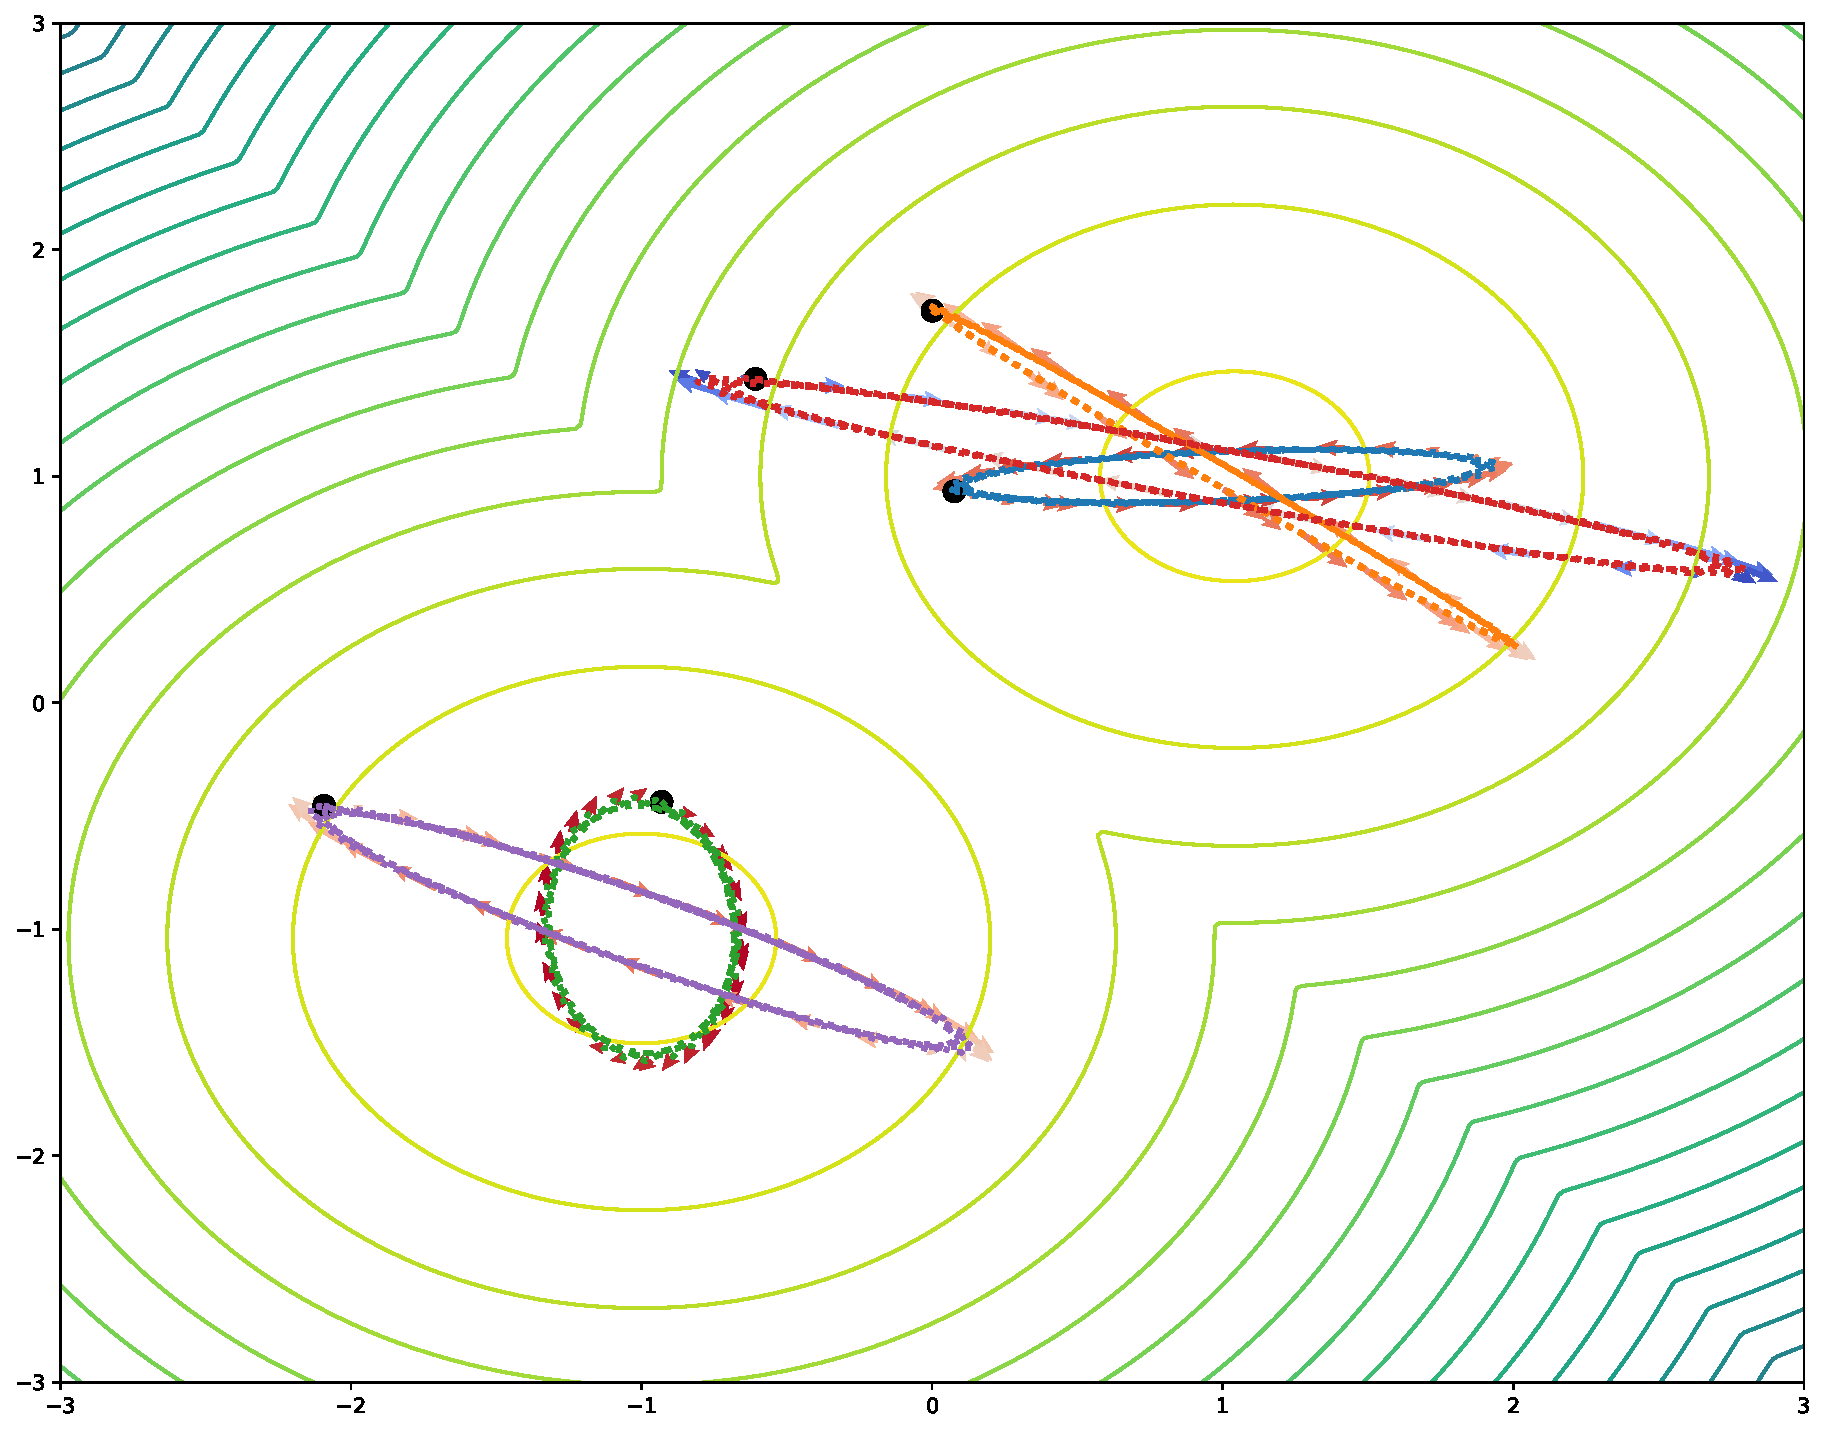
\includegraphics[width=0.25\linewidth]{pics/gamma0.0K30h0.1.pdf} & \includegraphics[width=0.25\linewidth]{pics/gamma0.3K30h0.1.pdf} & 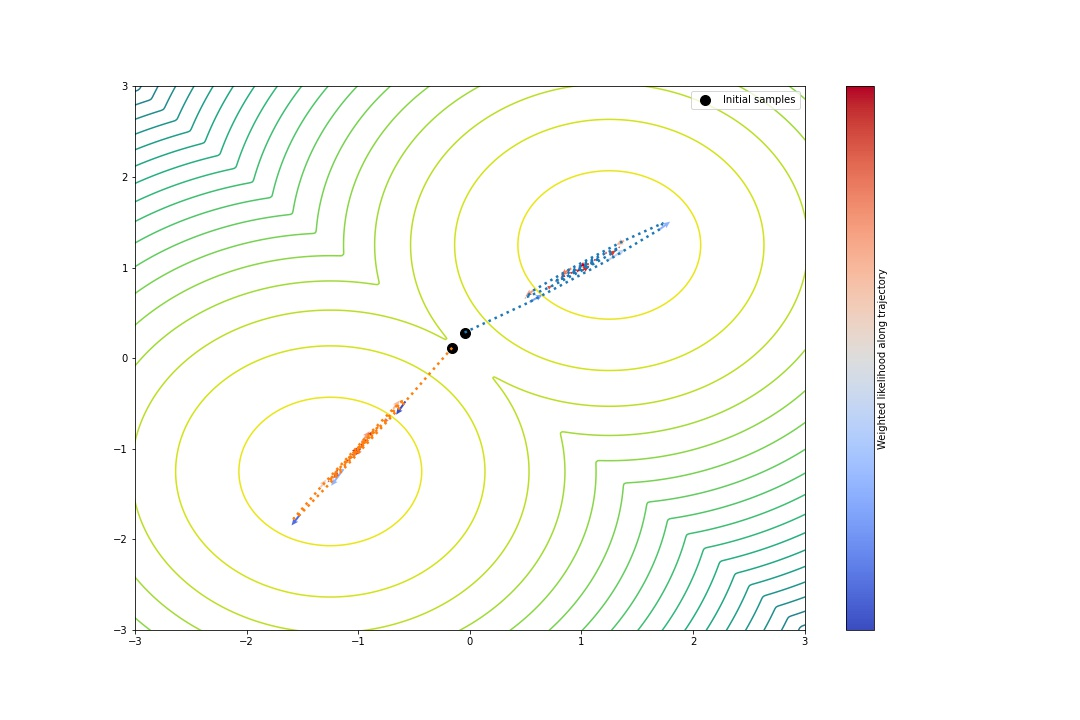
\includegraphics[width=0.25\linewidth]{pics/gamma2.0K30h0.1.pdf} &
     %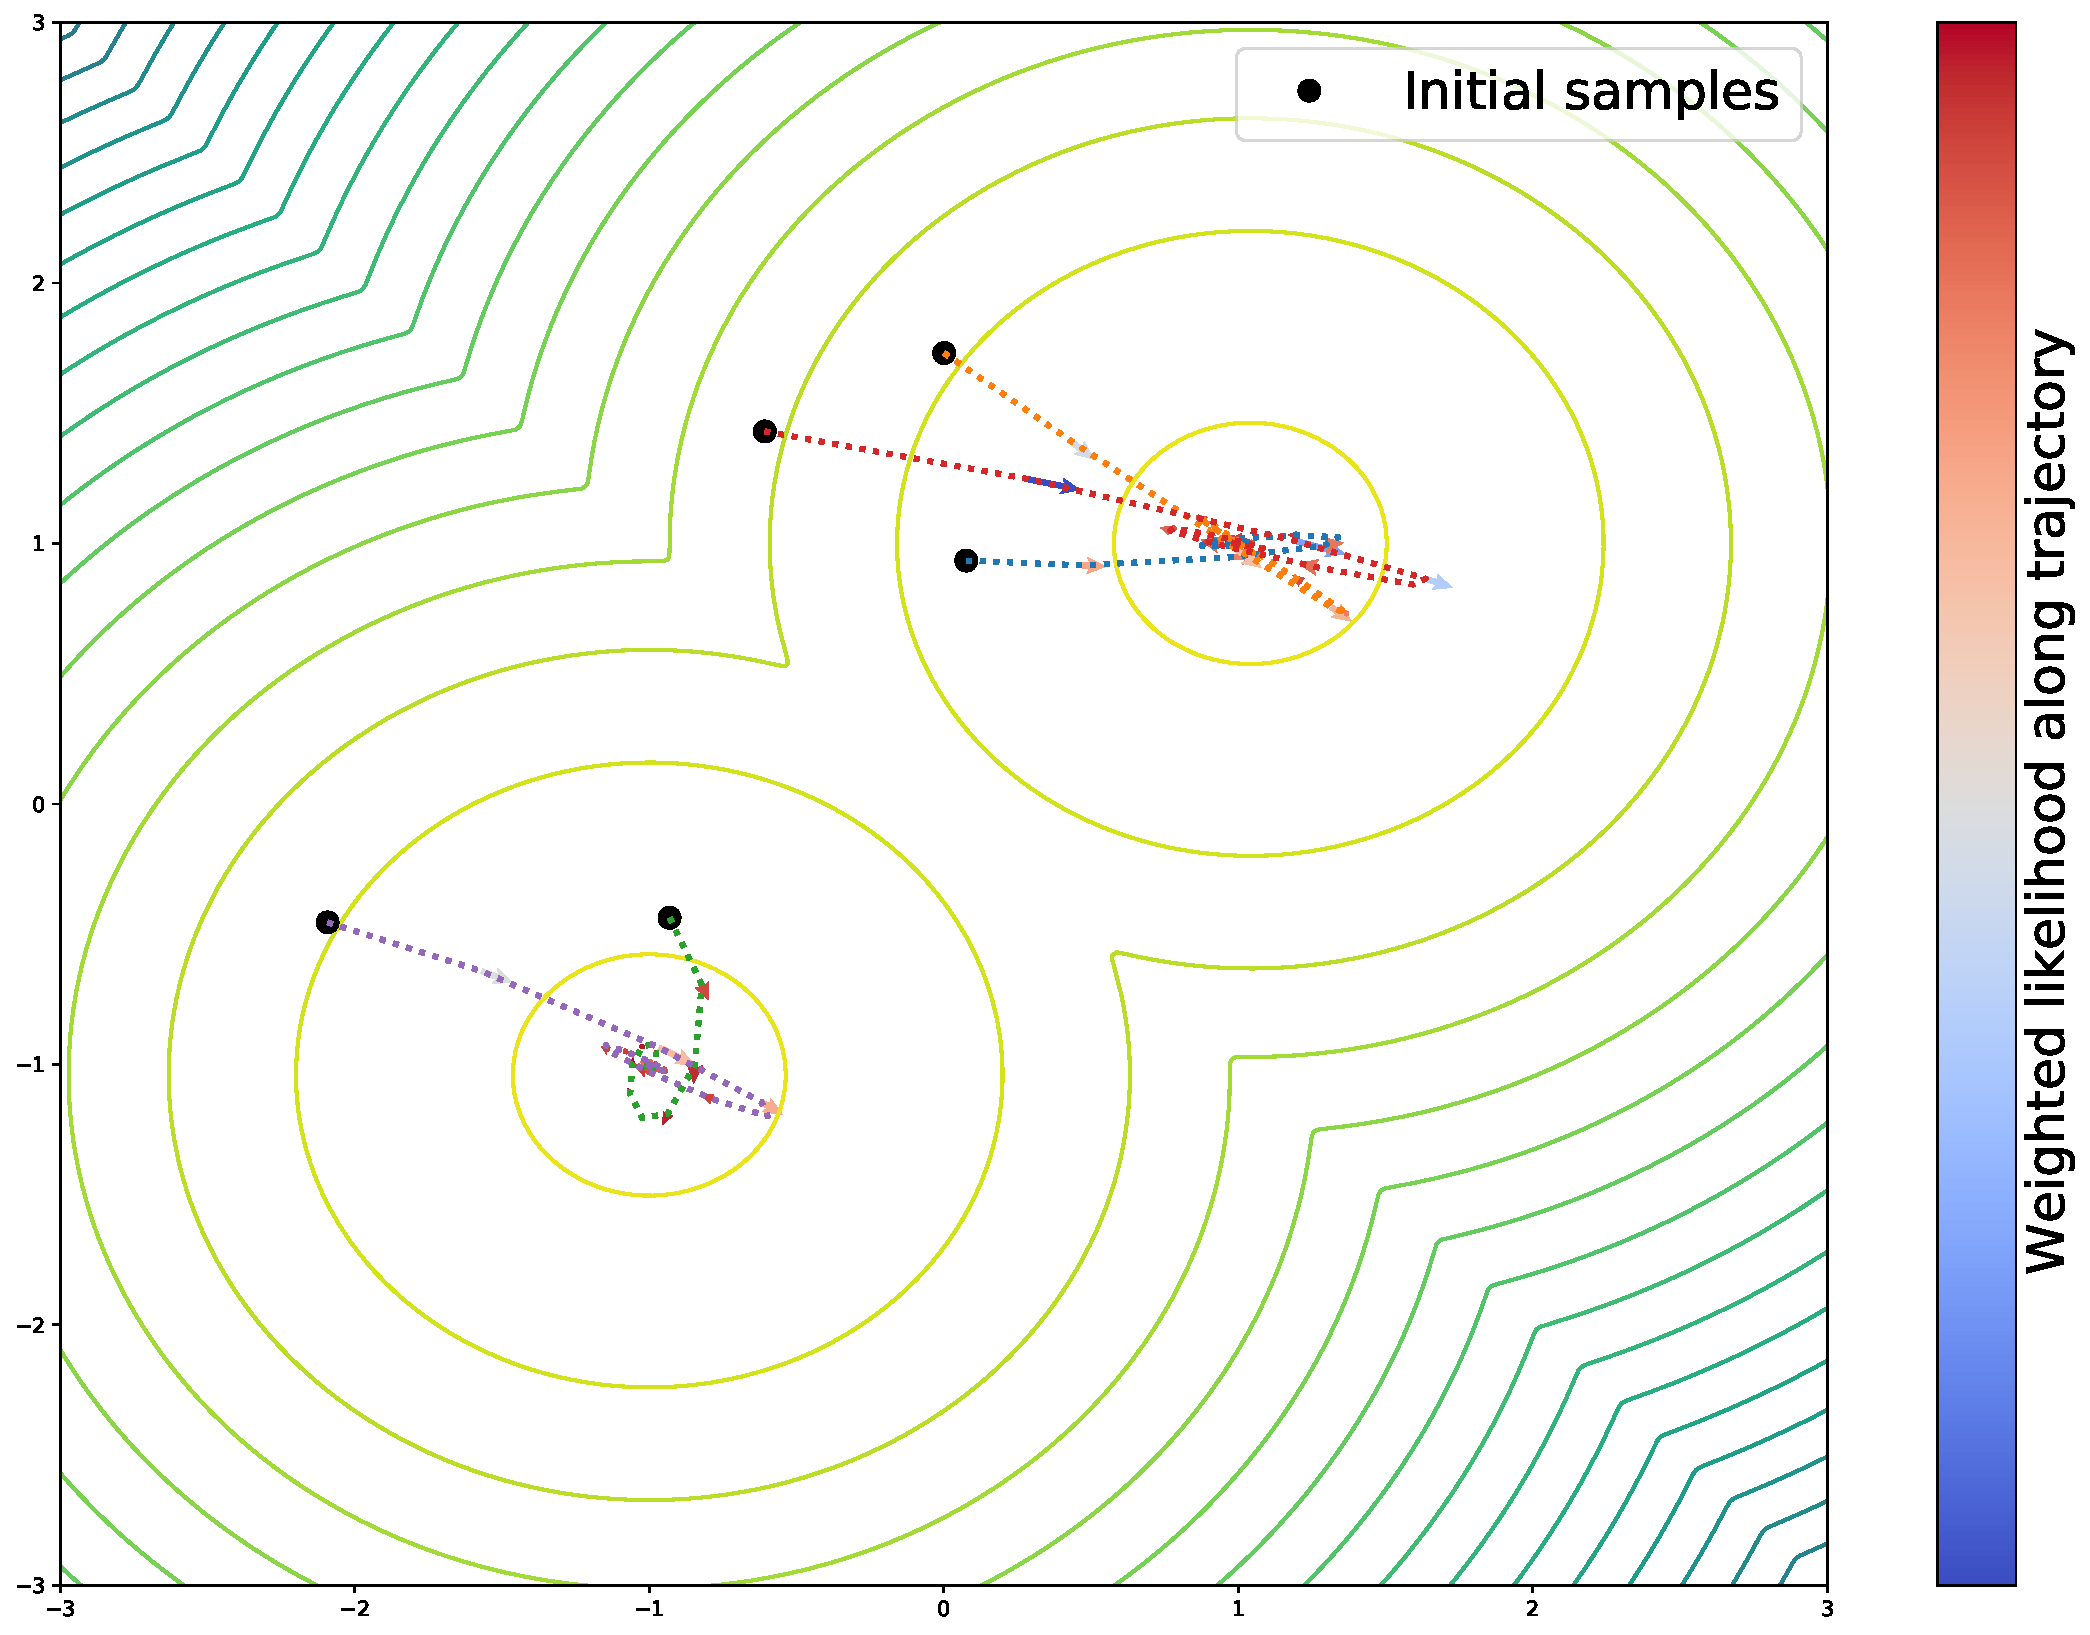
\includegraphics[width=0.25\linewidth]{pics/gamma5.0K30h0.1.pdf}
     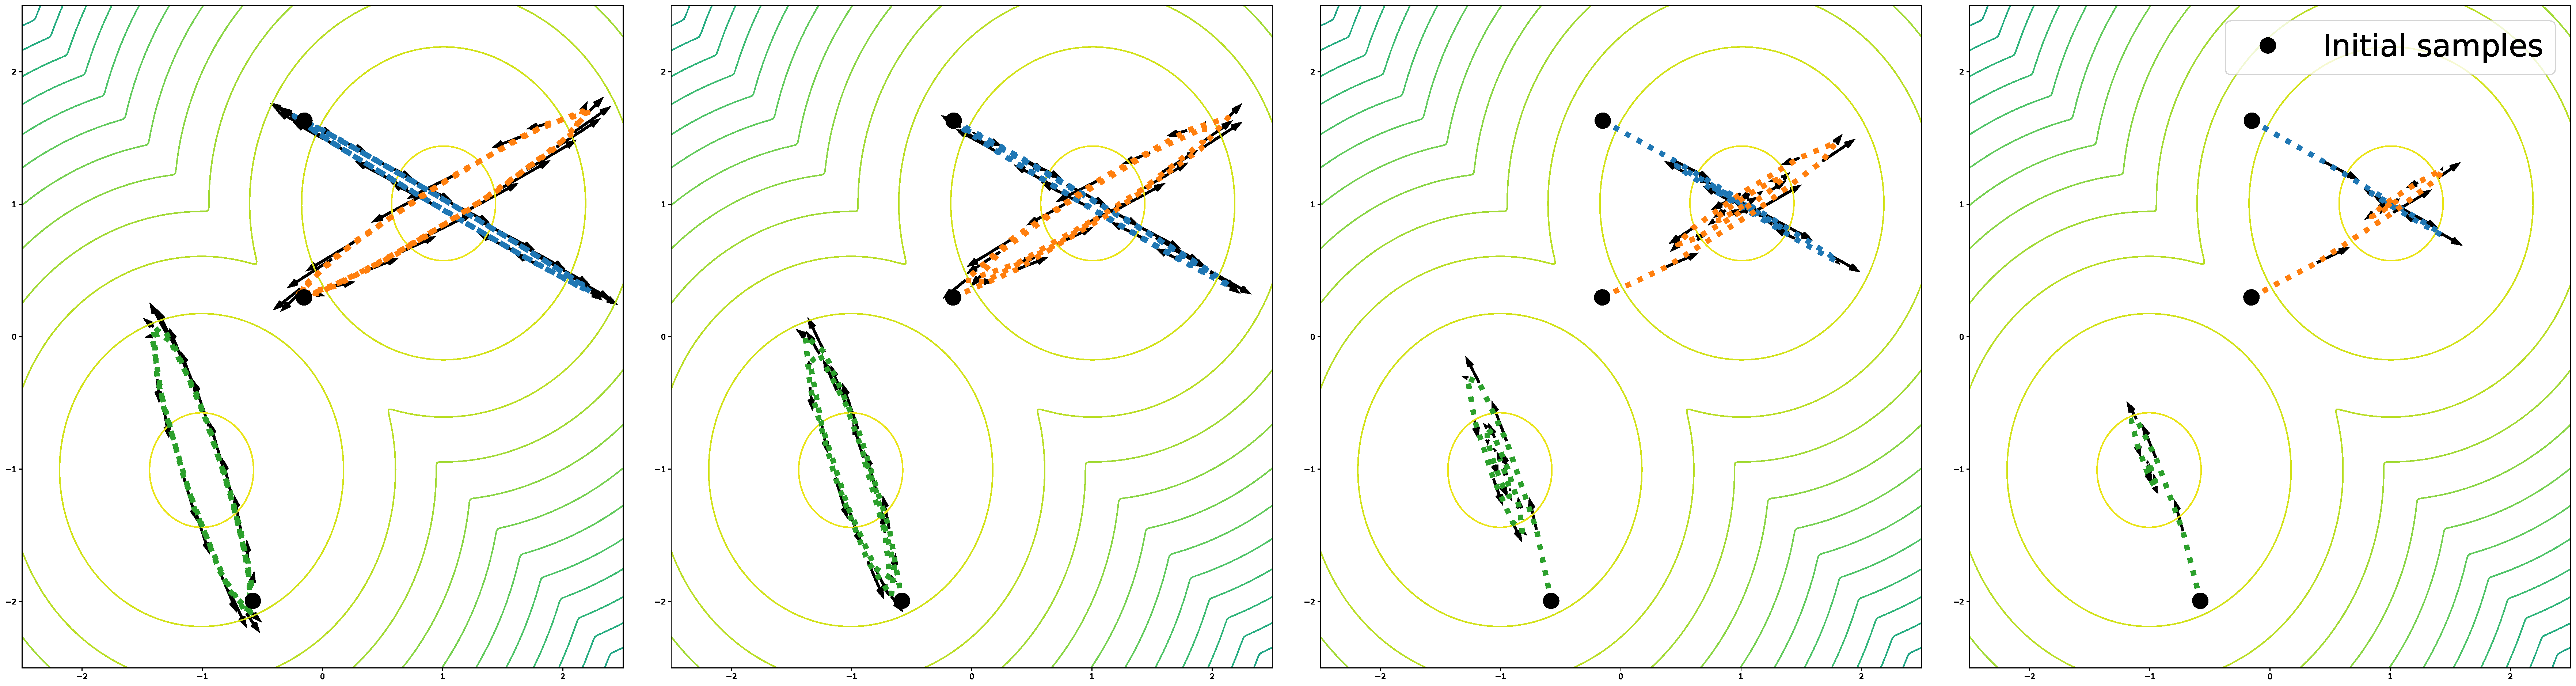
\includegraphics[width=1.0\linewidth]{pics/bigplot.pdf}
\end{tabular}
     \caption{Visualization of trajectories on a target of a mixture of two Gaussians given different Hamiltonian parameters. From left to right, $\gamma$ increasing from 0 to 0.3, 2 and 5.}
     \label{fig:toy_example_posterior}
 \end{figure*}
In the applications below, we consider the dissipative version of the symplectic Euler method of \eqref{eq:ODE_hamiltonian}, see \cite{francca2019conformal}.
This integrator can be constructed as a splitting  rendering of the two dissipative and conservative parts of the system \eqref{eq:ODE_hamiltonian}. When composing a dissipative with a  symplectic operator, we define for all $(q,p) \in \rset^{n}$, $\transfo_h$ by
%\begin{equation*}
 %\label{eq:def_psi_h}
\[\transfo_h(q,p) = (q+h\mass\{ \rme^{-h\gamma} p -h \nabla U(q)\}, \rme^{-h \gamma } p -h \nabla U(q))\eqsp, \] where $h >0$ is a stepsize. 
Indeed, this transformation can be shown to exactly recover the classical momentum optimization scheme, see \citep[Section 4]{francca2019conformal}. 
By \citep[Theorem 2]{francca2019conformal}, for any $h >0$ and $x \in \rset^{n}$,
$\JacOp{\transfo_h}(x) = \rme^{-\gamma h d}$. In addition, $\transfo_h$ is a $\rmC^1$-diffeomorphism with inverse given for any
$(p,q) \in \rset^{n}$ by $  \transfo_h^{-1}(q,p) = (q-h\mass p,\rme^{\gamma h}\{p+h \nabla
U(q-h\mass p)\})$.
% \begin{equation}
%   \label{eq:def_phi_h_inverse}
%  \eqsp.
% \end{equation}
Therefore, the weights of the  \IFIS\  estimator are given by
\begin{equation} 
w_{h,k}(x) = \frac{ \tilde \rho(\transfo^k_h(x)) \rme^{-\gamma k h d} }{
    \sum_{j = k-K}^k  \tilde \rho(\transfo^j_h(x)) \rme^{-\gamma j h d} },
\end{equation}
where $\tilde \rho(x) \propto \rho(q) e^{-K(p)}$.
The choice of the parameters $h$ and $\gamma$ is crucial and depends on the problem at stake. Moreover, the covariance matrix  $\mass$ is  auxiliary, but must be chosen carefully with respect to the application considered. In the applications below, $\mass$ is chosen classically as a diagonal covariance matrix, which is an additional parameter of the \IFIS\ estimator, see the  discussion  in \Cref{subsec:estim_constant}.



